\documentclass{standalone}
\usepackage{tikz}

\def\code#1{\textcolor{blue}{\textit{#1}}}

\begin{document}
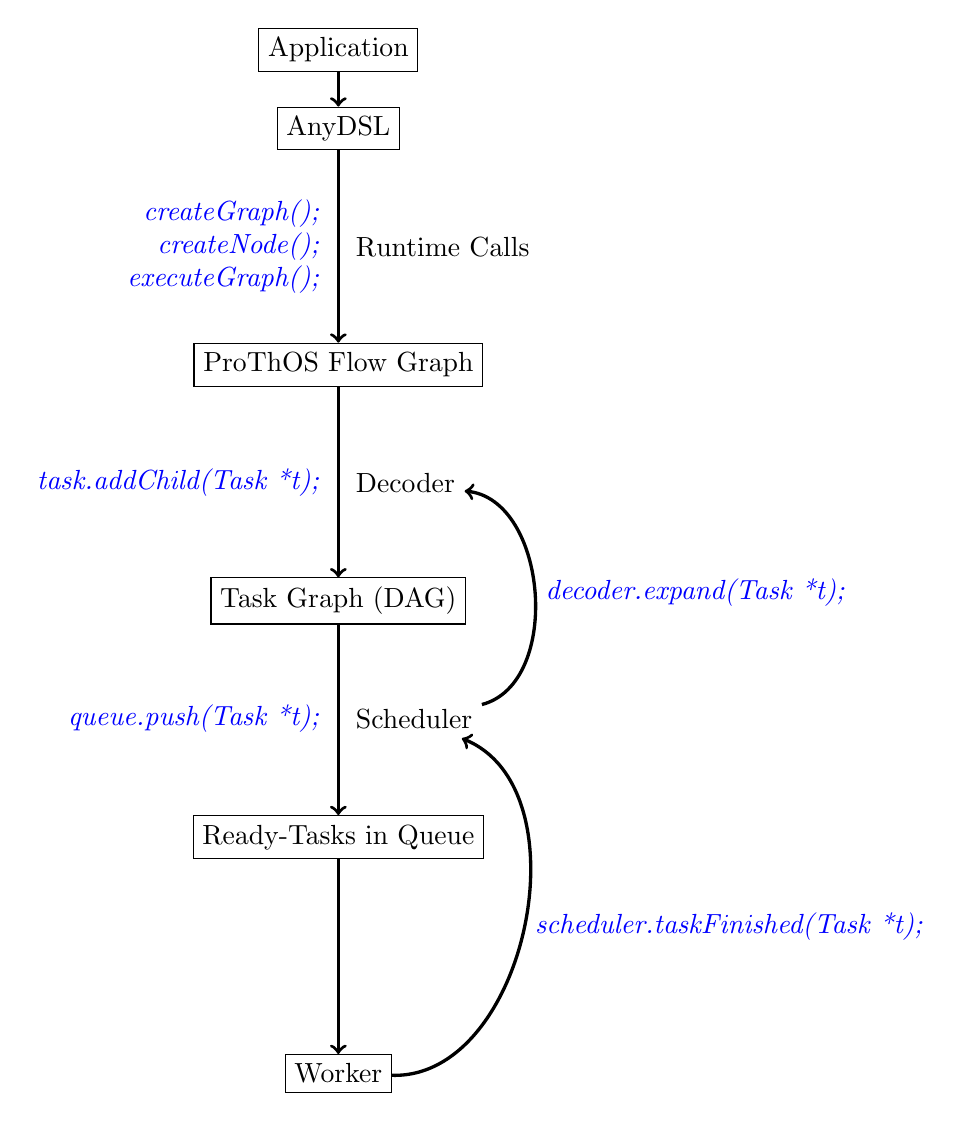
\begin{tikzpicture}[node distance =1cm]
\node (APP) at (0,4) [draw] {Application};
\node (ADSL) at (0,3) [draw] {AnyDSL};
\node (RTECALL) at (0.1,1.5) [anchor=west, align=left] {Runtime Calls};
\node at (-0.1,1.5) [anchor=east, align=right] {\code{createGraph();}\\ \code{createNode();}\\ \code{executeGraph();}};
\node (PFG) at (0,0) [draw] {ProThOS Flow Graph};
\node (Decoder) at (0.1,-1.5) [anchor=west, align=left] {Decoder};
\node at (-0.1,-1.5) [anchor=east, align=right] {\code{task.addChild(Task *t);}};
\node (TG) at (0,-3)[draw] {Task Graph (DAG)};
\node (Sched) at (0.1,-4.5) [anchor=west, align=left] {Scheduler};
\node at (-0.1,-4.5) [anchor=east, align=right] {\code{queue.push(Task *t);}};
\node (RTQ) at (0,-6) [draw] {Ready-Tasks in Queue};
\node (W) at (0,-9) [draw] {Worker};


\draw [->, very thick, draw] (APP) to (ADSL);
\draw [->, very thick, draw] (ADSL) to (PFG);
\draw [->, very thick, draw] (PFG) to (TG);
\draw [->, very thick, draw] (TG) to (RTQ);
\draw [->, very thick, draw] (RTQ) to (W);
\path [->, very thick] (Sched) edge [bend right=80] node[anchor=west] {\code{decoder.expand(Task *t);}} (Decoder);
\path [->, very thick] (W) edge [bend right=80] node[anchor=west] {\code{scheduler.taskFinished(Task *t);}} (Sched);
\end{tikzpicture}
\end{document}
